%% LyX 2.0.2 created this file.  For more info, see http://www.lyx.org/.
%% Do not edit unless you really know what you are doing.
\documentclass[10pt]{article}
\usepackage[T1]{fontenc}
\usepackage[utf8x]{inputenc}
\usepackage{geometry}
\geometry{verbose,tmargin=2.5cm,bmargin=2.5cm,lmargin=2cm,rmargin=1.5cm,headsep=0.5cm,footskip=1cm}
\usepackage{color}
\usepackage{amsmath}
\usepackage{amssymb}
\usepackage{graphicx}
\usepackage{setspace}
\doublespacing
\usepackage[unicode=true,pdfusetitle,
 bookmarks=true,bookmarksnumbered=true,bookmarksopen=true,bookmarksopenlevel=1,
 breaklinks=false,pdfborder={0 0 1},backref=section,colorlinks=true]
 {hyperref}
\hypersetup{
 urlcolor=blue,citecolor=blue}

\makeatletter

%%%%%%%%%%%%%%%%%%%%%%%%%%%%%% LyX specific LaTeX commands.
%% Because html converters don't know tabularnewline
\providecommand{\tabularnewline}{\\}

%%%%%%%%%%%%%%%%%%%%%%%%%%%%%% User specified LaTeX commands.
\@ifundefined{definecolor}
 {\usepackage{color}}{}
\@ifundefined{definecolor}{\usepackage{color}}{}
\@ifundefined{definecolor}{\usepackage{color}}{}
\@ifundefined{definecolor}{\usepackage{color}}{}
\@ifundefined{definecolor}{\usepackage{color}}{}
\@ifundefined{definecolor}{\usepackage{color}}{}
\@ifundefined{definecolor}{\usepackage{color}}{}
\@ifundefined{definecolor}{\usepackage{color}}{}
\@ifundefined{definecolor}{\usepackage{color}}{}
\@ifundefined{definecolor}{\usepackage{color}}{}
\@ifundefined{definecolor}{\usepackage{color}}{}

%\usepackage[french]{babel}
\usepackage{booktabs}\usepackage[format=plain,labelsep=endash,labelfont=bf]{caption}


 %\linenumbers

\makeatother

\begin{document}

\title{Reference Document for Giang's Ph.D. Subject}


\date{31/10/2014 Version 1.1}


\title{Quantifying the effect of synchrony on the persistence of infectious
diseases in a metapopulation}


\author{Tran Thi Cam Giang, Marc Choisy, Jean-Daniel Zucker}
\maketitle
\begin{abstract}
Global persistence of infectious diseases is a big problem for epidemiologists.
Studies have showed that there are a lot of reasons to answer why
many communicable diseases still exist and have been developed in
more dangerous form. The asynchrony and the recolonization among subpopulations
are two key reasons pointed out. However, why these are the asynchrony
and the recolonozations in a metapopulation is still an open question.
Here we study the combined effects of forcing phase heterogeneity
in the seasonally forced contact rate on global persistence of disease.
We carry out an exploitation of stochastic dynamics in a susceptible-exposed-infectious-recovered
(SEIR) model of the spread of infectious diseases in a metapopulation
of n subpopulations. Starting with continuous-time Markov description
of the model of deterministic equation, the direct method of Gillespie(1977)
\cite{gillespie1977exact} in the class of Monte-Carlo simulation
methods allows us to simulate exactly the spread of disease with the
SEIR model. Our finding of the exploitation of stochastic dynamics
points out that the persistence of the disease in the meta-population
is characterized as an exponential survival model on data simulated
by the stochastic model. Using a parametric survival model for an
exponential distribution (R package 'survival' \cite{survival-package}),
we estimate the global extinction rate which represents the global
persistence of disease in the meta-population. We find how bigger
the forcing phase heterogeneity becomes, and how larger the global
persistence gets.

\textbf{Keywords}: SEIR model, Markov chain, Monte-Carlo simulation
methods, spatial synchronization, disease persistence, meta-population. 
\end{abstract}

\section{INTRODUCTION}

News about infectious diseases has always been a subject of worry
to parents as well as all. It has brought many problems to humain
society. Recent works have shown that infectious diseases do spread
in space \cite{Cumming2004,Grenfell2001,Smith2004,viboud2006synchrony}.
The exact form of disease movement depends on a number of local factors
(demographic including population size \cite{Hagenaars2004}, growth
rate and death rate \cite{Conlan2007}, sociological such as school
period of children, work tendency from rural to urban, environmental
and climatic comprising seasonal variations in seasonality \cite{Conlan2010,Griffen2009},
temperature and rainfall, immunological for diseases, etc...) as well
as the connections between the different populations (i.e. spatial
structure) \cite{Yan2007} such as distance \cite{Hagenaars2004},
coupling rate, number of individuals between populations, etc....Hence,
we focus on spread of disease in space by using variations in the
seasonal aspects of subpopulations and after examine how synchrony
could affect the persistence of infectious diseases in a metapopulation.

In modeling of ecological system, presenting interactions between
humans, subpopulations, geographic conditions and the metapopulation
model is a good choice. Metapopulation is a set of subpopulations
with mutual interaction \cite{Levins1969} here a subpopulation can
only go extinct locally and be recolonized by another after it is
emptied by extinction \cite{Bolker1996,Hanski1998,Levins1969}. It
is the reason that the ecological theory of metapopualtion can point
out that the persistence of a population depends on the dynamics of
migrations between the different sub-populations of the metapopualtion
\cite{Hagenaars2004,Hanski1998,Hanski2004,Levins1969}. The “colonization”
caused by migrations brings infection to an uninfected subpopulation
and we call infected individuals colonizers.

In addition, the disease persistence capability in a metapopulation
depends positively on level of synchrony/asynchrony between subpopulations
\cite{Hagenaars2004,Heino1997}. Many studies showed that the synchronization
of epidemics in all asynchronous subpopulations causes the recolonization
of diseases for locally extinct subpopulation \cite{Bolker1996,Hagenaars2004,Hanski1998,Heino1997,Yaari2012}.
So, the recolonization becomes the main reason for which disease persistence
exists. The disease always appears in metapopulation if and only if
there is at least one non-extinct subpopulation.\textbf{ }In 1996\textbf{,
}in order to explain why measles persists after lot of vaccination
policies, Bolker \cite{Bolker1996} used the measles data before and
after vaccination from 1964 to 1988 in England and Wales. Vaccination
has broken high synchrony between the UK cities in prevaccination
era, and at the same time, causes decorrelation and enhances global
persistence of the infection, because of decorrelating factors of
vaccination such as the starting moment of vaccination policies, number
of susceptibles vaccinated and interaction between vaccination policies
\cite{Bolker1996,Rohani1999}. A decrease in correlation between subpopulations
may make a metapopulation more difficult to eradicate infectious diseases\textbf{
}\cite{Bolker1996,Earn1998}. In addition, the level of synchrony
between the subpopulations is strongly governed by the migration rate
and distances between them \cite{Heino1997}. In our modern world,
the distance problem isn't large anymore for individuals who want
to travel. There are a lot of cities very remote, but very connected,
and thus very synchronous as in the USA \cite{Choisy2012}. In contrast,
migration among subpopulations has become a big problem. The disease
synchrony speed within a metapopulation can strongly increase when
migration rate there is strong \cite{KeelingRohani2008}.\textbf{
}The migration rates are directly proportional to the amount of variation
in metapopulation size, but inversely to the amount of variation in
subpopulation size, over time \cite{Dey2006,Griffen2009}. So, migration
is key to the recolonization of empty subpopulation and simultaneously
increases the degree of synchrony between subpopulations in spatially
structured metapopulation. However, the vast majority of infectious
diseases control policies that are applied in the world are still
based on rationales that do not consider the local extinction/recolonization
dynamics. This is maybe a reason why measles persists\textbf{ }around
the world, despite highly local vaccine coverages \cite{Conlan2007}.
For example, in the start of the 2014, the World Health Organization
(WHO) had officially stated the global measles epidemic outbreak.
In the first three months of the year 2014, there were about 56,000
cases of measle infections in 75 countries \cite{WHO2014a}, including
countries in south-east Asia and most particularly, Vietnam \cite{http://healthmap.org/site/diseasedaily/article/measles-reemerges-vietnam-22814}.
We discovered measles persistence in the world for many years without
extinction, from one nation to another as well as from cities to other
cities. Though the moment of disease outbreaks in each region differs.
For neighbouring regions with disease persistence, there is a time-lag
differs between disease outbreak. This is explained in sociology by
difference in culture, in geographic condition and more particularly
seasonality.

Seasonality has been one in rather robust ingredients influencing
the disease persistence process. Seasonal changes can alter migration
tendency between urban and rural areas \cite{Ferrari2010}, also residence
time of hosts, vectors and pathogens. Seasonal variation can thus
determine population size, migration and interaction capabilities
and particularly infection rate at which susceptible individuals become
infected \cite{Altizer2006,Hosseini2004}. Hence, infectious disease
outbreak occurs due to this infection rate. However, finding a clear
mechanism of seasonal forcing for modelling is a very difficult work
because of unidentified formula for seasonal forcing \cite{Altizer2006,Ferrari2010}.
For indirectly transmission diseases such as water-born and vector-born,
finding seasonality characteristics is less a problem, however, in
direct contrast to transmission diseases such as measles. Seasonal
forcing in a metapopulation is influenced by weather and climate in
region, school schedule of children, and rural-urban migration in
countries \cite{Bolker1995,Conlan2007,Ferrari2010,Gunning2013}. In
these factors, the seasonal aggregation of children in primary schools
affects clearly the infection rate in metapopulation. The infection
rate decreases due to children holidays but is inverse when the children
come back to school \cite{Conlan2007}.\textbf{ }So\textbf{, }exploring
the influence of seasonality for the infection rate $\beta$ in simulation
has been developed in many previous years. If the infection rates
given are the same in all subpopulations, so this metapopualtion model
is a rather simple model \cite{Rozhnova2012,Rozhnova12013} and the
symmetry of the fixed points among subpopulations will not be broken.
In contrast, if the infection rate is different in all subpopulations,
so we have a more complex oscilation metapopulation model, but close
to the oscilations in reality. Thus, realizing the oscilations of
infectious diseases in life within metapopulation simulation models
to estimate global disease persistence time has become a large problem
and the infectious disease eradication has become our aim\textbf{
}\cite{Earn1998}.

Here we propose a simulation study to quantify the effect of synchrony
on the persistence of infectious diseases. We use stochastic simulations
for infectious diseases in a metapopualtion, then we consider different
spatial structures from the simplest to more complex. These forcings
can reflect local demographic, sociological, environmental, or climatic
factors. The level of synchrony is computed from the phases of forcing
in the different subpopulations and persistence is quantified by using
statistical tools from survival analysis. Here, we are concerned about
measles and simultaneously use the parameter values from articles
and measles reports. As the persistence of measles has been largely
studied in the literature and its still unexplained while global persistence
is a growing concern for WHO and public health authorities around
the world \cite{Conlan2010}.

To do this, we first build the deterministic model for a metapopualtion.
Then, we describe the spatial structure and the stochastic version
of the model. Finally, we introduce the characterization of global
persistence in the metapopulation based on the measles characteristics.


\section{MATERIAL AND METHODS }


\subsection{MATERIAL}


\subsubsection{Deterministic model for many subpopulations}

The standard SEIR model (susceptible-exposed-infective-recovered)
has been strongly developed for the dynamics of directly infectious
disease \cite{Bolker1995}. For disease-based metapopulation models,
we give here a suitable new version of the SEIR equation that would
be as follows:

Consider a metapopulation of $n$ sub-populations. In a subpopulation
$i$ of size $N_{i}$, disease dynamics can be deterministically described
by the following set of differential equations \cite{Anderson&May1992}:

\begin{eqnarray}
\frac{dS_{i}}{dt} & = & \mu N_{i}-\lambda_{i}S_{i}-\mu S_{i}\label{eq:dS}\\
\frac{dE_{i}}{dt} & = & \lambda_{i}S_{i}-\mu E_{i}-\sigma E_{i}\\
\frac{dI_{i}}{dt} & = & \sigma E_{i}-\mu I_{i}-\gamma I_{i}\label{eq:infectieux}\\
\frac{dR_{i}}{dt} & = & \gamma I_{i}-\mu R_{i}\label{eq:dR}
\end{eqnarray}
 where $S_{i}$, $E_{i}$, $I_{i}$ et $R_{i}$ are the numbers of
susceptible, exposed, infectious and recovered in this sub-population
$i$ respectively. Individuals are born susceptible, die at a rate
$\mu$, become infected with the force of infection $\lambda_{i}$,
infectious after a latency period of an average duration of $1/\sigma$
and recover at the rate $\gamma$. In a case the infectious contact
rate is constant, the equilibrium values of the variables $S$, $E$,
$I$ and $R$ can be expressed analytically (see appendix). The force
of infection depends not only on the total population size $N_{i}$
and the number of infected $I_{i}$ in subpopulation $i$, but also
in other sub-populations \cite{KeelingRohani2008} :

\begin{equation}
\lambda_{i}=\beta_{i}\frac{I_{i}}{N_{i}}+\sum_{\substack{j=1\\
j\neq i
}
}^{n}\rho_{ij}\left[\frac{\beta_{i}\text{[}(1-\varepsilon_{ij})I_{j}-I_{i}]}{N_{i}}+\frac{\varepsilon_{ij}\beta_{j}I_{j}}{N_{j}}\right]\label{eq:force-1}
\end{equation}
 where $\beta_{i}$ is the contact rate in population $i$ and $\rho_{ij}=\rho_{ji}$
($0\leqslant\rho_{ij}\leqslant1$ and $\rho_{ii}=1$) is the coupling
between subpopulations $i$ and $j$. Among the infections caused
by contacts with infected from other subpopulations, $\varepsilon_{ij}=\varepsilon_{ji}$
($0\leqslant\varepsilon_{ij}\leqslant1$) is the proportion of infections
due to susceptible individuals visiting other populations as opposed
to infected individuals from other populations visiting the focal
population. See appendix for detail on the construction of this equation.
We can verify that in the limit case on one single subpopulation in
the metapopulation ($i=j$ and $n=1$) we have 
\begin{equation}
\lambda_{i}=\beta_{i}\frac{I_{i}}{N_{i}}.
\end{equation}
 Consider that the contact rate $\beta_{i}$ is seasonally forced
\cite{Altizer2006} and seasonality is an annually periodic function
of time \cite{Grenfell1995}. As a result, 
\begin{equation}
\beta_{i}(t)=b_{0}\left[1+b_{1}\cos\left(\frac{2\pi t}{T}+\varphi_{i}\right)\right]\label{eq:beta_i}
\end{equation}
 where $t$ is the time, $b_{0}$ and $b_{1}$ are the mean value
and amplitude of the infection rate $\beta$ at which susceptible
individuals become infected, $T$ and $\varphi_{i}$ are the period
and the phase of the forcing. With the annual sinusoidal form of the
infection rate, we really have the sinusoidally forced SEIR metapopulation
model.


\subsubsection{Stochastic model for many subpopulations}

In order to study the persistence of the disease, we must consider
a stochastic version of the model \cite{Keeling2002,Lloyd2001,renshaw1993modelling}.
We use for that a population-based time-to-next-event model based
on Gillespie's algorithm \cite{gillespie1977exact}. Table \ref{tab:stoch_ev}
lists all the events of the model, occurring in subpopulation $i$.

\begin{table}[tbph]
\begin{centering}
\caption{\label{tab:stoch_ev}Events of the stochastic version of the model
of equations \ref{eq:dS}-\ref{eq:dR}, occuring in subpopulation
$i$.}

\par\end{centering}

\centering{}%
\begin{tabular}{lcc}
\toprule Events  & Rates  & Transitions \tabularnewline
\midrule birth  & $\mu N_{i}$  & $S_{i}\leftarrow S_{i}+1$ and $N_{i}\leftarrow N_{i}+1$ \tabularnewline
death of a susceptible  & $\mu S_{i}$  & $S_{i}\leftarrow S_{i}-1$ \tabularnewline
death of an exposed  & $\mu E_{i}$  & $E_{i}\leftarrow E_{i}-1$ \tabularnewline
death of an infected  & $\mu I_{i}$  & $I_{i}\leftarrow I_{i}-1$ \tabularnewline
death of an immune  & $\mu R_{i}$  & $I_{i}\leftarrow I_{i}-1$ \tabularnewline
infection  & $\lambda_{i}S_{i}$  & $S_{i}\leftarrow S_{i}-1$ and $E_{i}\leftarrow E_{i}+1$ \tabularnewline
becoming infectious  & $\sigma E_{i}$  & $E_{i}\leftarrow E_{i}-1$ and $I_{i}\leftarrow I_{i}+1$ \tabularnewline
recovery  & $\gamma I_{i}$  & $I_{i}\leftarrow I_{i}-1$ and $R_{i}\leftarrow R_{i}+1$ \tabularnewline
\bottomrule  &  & \tabularnewline
\end{tabular}
\end{table}



\subsubsection{Spatial structures}

A metapopulation is a population of populations (subpopulations).
Such a structure implies an heterogeneity in the sense where the probability
of contact (or contact rate) between individuals from a same subpopulation
is higher than the probability of contact between individuals of different
subpopulations \cite{Hanski2004}. Such heterogeneity is actually
the result of the interaction between two phenomena that are often
difficult to disentangle in nature. The first one relates to the granularity
of the metapopulation (as rendered by the number of and sizes of subpopulations)
and the second one relates to the isolation between subpopulations
(as can be rendered, among others, by physical distances separating
each pair of subpopulations). Moreover, according to the findings
of Benjamin Bolker (1995) \cite{Bolker1995}, there is no coexistence
between periodicity and disease persistence in non-spatial measles
models, and spatial structure is an important factor to both enhance
persistence and create new types of dynamic behaviour.

In order to identify clearly the causes of observed phenomena, these
two aspects will be modeled distinctly. In this article, our null
model (model 0) will be a metapopulation without any explicit spatial
distance (all the subpopulations are at the same distance from each
other) and where all the subpopulations have the same population size
$N$. Like the original Levins's model \cite{Levins1969}, this model
considers that all the subpopulations are at equal distance from each
other: 
\begin{equation}
\rho_{ij}=\rho,\qquad0\leqslant\rho\leqslant1,\qquad\forall i,\forall j.
\end{equation}
 The structure of this metapopulation is thus characterized by 3 parameters:
(i) the number $n$ of sub-populations, (ii) the population size $N$
($N_{i}=N$, $\forall i$) of all these subpopulations and, (iii)
the coupling (or distance) $\rho$ between these subpopulations.


\subsection{METHOD}


\subsubsection{Global persistence in a metapopulation}

In order to examine questions of interaction between disease transmissibility
and phase of seasonal forcing, we start in this section by studing
the stochastic SEIR model in a metapopualtion of $n$ subpopulations.
For this meta-population, we observe the disease extinction in time
due to spatial synchrony/asynchrony that are influenced by phase difference
in seasonal forcing. To create the phase difference, we change the
value of the forcing phase for each city. In this experience, we use
a parameter $\varphi_{max}$ in radian that runs in the interval from
zero to $\pi$. With each value of $\varphi_{max}$, based on \textbf{$n$}
the number of subpopulations in the metapopulation, we divide the
interval {[}0, $\varphi_{max}${]} into a set of (n-1) equal samples,
so the value of the forcing phase of the $i^{th}$ subpopulation is
correspondent to $i^{th}$ value in the set. We call $\varphi_{max}$
asynchrony parameter.

The persistence of disease in the metapopulation was characterized
by fitting an exponential survival model \cite{Conlan2010,Kleinbaum2005}
on data simulated by the stochastic model\textbf{.} To measure the
persistence in ecology and epidemiology, so many methods we can use
\cite{Conlan2010,Gunning2013,Keeling2002}. For example, Keeling et
al.(2002) \cite{Keeling2002} gave two methods. One method was for
an isolated metapopulation without migration by calculating the expected
extinction time or the extinction rate during a given period. This
was a theoretical measure as no real data exists to compare with model
results. The other method for a population with migration was found
by calculating the number or the total duration of extinctions. Then
in 2010, ``mean annual fade-out'' and ``fade-outs post epidemic''
methods proposed by Conlan \cite{Conlan2010} were used to quantify
persistence by basing on the proportion or on the frequency of zero
reports in a given reporting interval. For our metapopulation of $n$
subpopulations, to do so we run first $m$ independent simulations
of our stochastic model. We calculate then the average metapopulation
size by summing subpopulations at each sample time and averaging across
the entire time series for each metapopulation. Lastly, we record
the dates $t$ of global disease extinction in all these $m$ metapopulations.
These dates allow to draw Kaplan-Meier survival curves from which
we estimate the persistence rates $\chi$: 
\begin{equation}
M(t)=\exp(-\chi t)
\end{equation}
 where $M(t)$ ($0\leqslant M(t)\leqslant m$) is the number of metapopulations
in which the disease is not extinct at time $t$.

To assess global extinction rate as well as global persistence level
in metapopulation, here, we use the parametric survival model for
the exponential distribution (R package '$survival$' \cite{survival-package}).
Due to that, we can capture one of the most important features of
stochastic systems in spatial structure : its global persistence of
disease.

\bigskip{}



\subsubsection{Characterization of synchrony}

Call $\delta_{ij}=\delta_{ji}$ ($0\leqslant\delta_{ij}<2\pi$) the
phase difference between subpopulations $i$ and $j$ : 
\begin{equation}
\delta_{ij}=|\varphi_{i}-\varphi_{j}|\bmod2\pi
\end{equation}
 where $\varphi{}_{i}$ and $\varphi{}_{j}$ are the phases of the
contact rates (equation \ref{eq:beta_i}) in subpopulations $i$ et
$j$. Populations $i$ and $j$ are perfectly in phase if $\delta_{ij}=\delta_{ji}=0$
or $2\pi$ and in opposition of phase if $\delta_{ij}=\delta_{ji}=\pi$.
We can thus define the degree of synchrony $\xi_{ij}=\xi_{ji}$ ($0\leqslant\xi_{ij}\leqslant1$)
between populations $i$ and $j$ as 
\begin{equation}
\xi_{ij}=\left|1-\frac{\delta_{ij}}{\pi}\right|.
\end{equation}
 
\begin{figure}[htpb]
\centering 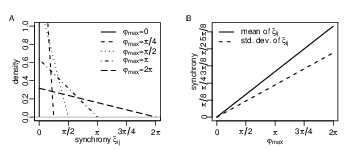
\includegraphics{figure1} \caption{\label{fig:synchrony-1}Synchrony in the case of model 0. (A) distribution
of synchrony $\xi_{ij}$ for various values of $\varphi_{max}$. (B)
mean and standard deviation of the distribution of $\xi_{ij}$ as
functions of $\varphi_{\mbox{\tiny max}}$.}
\end{figure}


Consider that in the metapopulation the phases $\varphi_{i}$ of the
contact rates in the $n$ subpopulations are evenly distributed between
0 and $\varphi_{\mbox{\tiny max}}$ ($0\leqslant\varphi_{\mbox{\tiny max}}\leqslant\pi$).
We can express the mean of the pairwise phase differences $\delta_{ij}=\delta_{ji}$
as 
\begin{equation}
<\!\!\delta_{ij}\!\!>\;=\;<\!\!\delta_{ji}\!\!>\;=2\varphi_{\mbox{\tiny max}}\sum_{k=1}^{n-1}\frac{(n-k)k}{(n-1)n^{2}}=\frac{n+1}{3n}\varphi_{\mbox{\tiny max}}
\end{equation}
 and thus the mean of the synchronies $\xi_{ij}=\xi_{ji}$ as 
\begin{equation}
<\!\!\xi_{ij}\!\!>\;=\;<\!\!\xi_{ji}\!\!>\;=1-\frac{n+1}{3n}\frac{\varphi_{\mbox{\tiny max}}}{\pi}
\end{equation}
 and thus 
\begin{equation}
\lim_{n\to\infty}<\!\!\xi_{ij}\!\!>\;=1-\frac{\varphi_{\mbox{\tiny max}}}{3\pi}
\end{equation}


This last result shows that, for a high enough number $n$ of subpopulations,
the mean value of the $\xi_{ij}$ does not depend on the number of
subpopulation.

The values of $\varphi_{i}$ are chosen so that they are uniformly
distributed between $\varphi_{\mbox{\tiny min}}=0$ and $\varphi_{\mbox{\tiny max}}$.
The distribution of $\xi_{ij}$ doesn't depend on $n$ the number
of subpopulation, but only depends $\varphi_{\mbox{\tiny max}}$ and
may be is characterized by one single parameter (we choose the average
value of all $\xi_{ij}$)\textbf{, }view figure \ref{fig:synchrony-1}.


\subsection{Plan of experience}

\textbf{In this section, we will describe our plan of experience to
quantifying the effect of synchrony on the persistence of infectious
diseases in a metapopulation. We have four big concerns that we must
verify.}


\subsubsection{Quantifying disease persistence in the simplest metapopulation }

Firstly, we are interested in the correlation between global disease
persistence time when the forcing phase of the infection rate $\beta$
in each subpopulation alters and the recolonization in metapopulation.
In order to simplify this concern, we start with the metapopulation
of two subpopulations. To have the two subpopulations in synchrony,
we choose $\varphi_{max}$= 0. It means that the forcing phase of
$subpopulation_{1}$ and $subpopulation_{2}$ are the same phase,
$\varphi_{1}=\varphi_{2}=0$. Thereby, the fluctuations of the contact
rate $\beta(t)_{1}$ and $\beta(t)_{2}$ are in the same annual sinusoidal
form\textbf{.} In contrast, to have the two subpopulations in asynchrony,
we create the phase difference or the phase lag between the subpopulations.
It means that we have created a metapopulation in heterogeneity. Here,
we choose $\varphi_{max}$$=\pi/2$ and $\varphi_{max}$$=\pi$. The
phase difference between the forcing phase of $subpopulation_{1}$
and $subpopulation_{2}$, for $\varphi_{max}$$=\pi/2$, is $\varphi_{1}=0$
and $\varphi_{2}=\pi/2$, then for $\varphi_{max}$$=\pi$, is $\varphi=0$
and $\varphi_{2}=\pi$, so the fluctuation of $\beta(t)_{1}$ is phase
lag for $\beta(t)_{2}$'s. Based on $\varphi_{max}$, we are successfully
buiding a complex disease metapopulation mode.


\subsubsection{Quantifying global persistence and asynchrony level $\varphi_{max}$}

We will exploit more strongly the role of asynchrony $\varphi_{max}$
for global disease persistence time in metapopulation. $\varphi_{max}$
is an important parameter that we use to break fixed points as well
as first fixed points at begining moments between subpopulations.
Our goal is to examine global persistence for each value of $\varphi_{max}$
in the metapopulation. Simply, we base on survival regression model
for global peristence curve at each different value $\varphi_{max}$
to estimate its global extinction rate. We start also with the metapopualtion
of $n$ subpopulations given and $\varphi_{max}$ from 0 to $\pi$.
It means that we increase level of phase difference from the $subpopulation_{1}$
to $subpopulation_{n}$. We deploy \textbf{$m$} the number of different
simulations. Then, we use survival analysis to quantify persistence
level at each value of $\varphi_{max}$ with confidence interval to
95\%.


\subsubsection{Influence of other parameters on global disease persistence}

This last experience is how the population size of subpopulation,
the coupling strength between subpopulations and the number of subpopulations
in the metapopulation affect the disease persistence as well as the
relation between the global disease persistence and the asynchrony
parameter $\varphi_{max}$. In order to present the effect of the
third parameter on the correlation of the two first parameters (global
persistence level and $\varphi_{max}$), we will use a gradient coefficient
for the trajectory of the correlation between global persistence and
$\varphi_{max}$.


\subsubsection{Stochastic metapopulation simulations}

In order to run simulations, we use the same values of all parameters
for all subpopulations. We use the Gillespie's direct algorithm \cite{gillespie1977exact}
for metapopulation model as described in the previous part. With the
SEIR metapopulation model, measles is modeled \cite{Anderson&May1992,Gunning2013}.\textbf{
}Moreover, in this work, we use also the values of parameters for
the measles to do experiences. We have a table of the convenient values
for parameters of measles as follows :

\begin{table}[tbph]
\begin{centering}
\caption{\label{tab:valuesofparameter} Some Disease Parameter Values for Measles
from the Literature\textbf{ }\cite{Bolker1995,Choisy2012,Conlan2010,Keeling1997,Keeling2002,KeelingRohani2008}}

\par\end{centering}

\centering{}%
\begin{tabular}{lcc}
\textbf{parameter }  & \textbf{description }  & \textbf{value}\tabularnewline
$\mu$  & birth and death rate per day  & $1/(70*365)$ \tabularnewline
$\beta_{0}$  & mean value of the infection rate $\beta$ per day  & $1250/365$\tabularnewline
$\beta_{1}$  & amplitude of the infection rate $\beta$  & $0.15$\tabularnewline
$\gamma$  & recovery rate per day  & $1/8$\tabularnewline
$\sigma$  & average exposed duration per day  & $1/5$\tabularnewline
$\rho$  & coupling rate  & \textbf{$10^{-4}-1.0$}\tabularnewline
$\varphi_{max}$  & synchrony parameter in radian  & $0-\pi$\tabularnewline
$N$  & population size of subpopulation (individual)  & $5000-500,000$\tabularnewline
$n$  & number of subpopulation  & $2-30$\tabularnewline
$t_{max}$  & simulation time (year)  & $50$\tabularnewline
 &  & \tabularnewline
\end{tabular}
\end{table}


Following the table in detail about the convenient values of parameters,
we will use them through all simulations. We start doing a simulation
from a initial random number. Then, we aggregate the daily data (number
of individuals in the suceptible, exposed, infected and recovered
groups) into one-day intervals, and use this as the time step in the
model.


\section{RESULT}


\subsection{Quantifying disease persistence in the simplest metapopulation}

We start quantifying global disease persistence in the metapopulation
of two subpopulations by examining degree of synchronization between
infected individuals in two connected subpopulations. This is the
simplest metapopulation, for which we can view easily the influence
of the level of synchrony on the disease persistence and recolonization
of disease in the metapopulation over time due to the asynchrony parameter
$\varphi_{max}$.

We chose here the metapopulation of two subpopulations, $N_{1}=N_{2}=300,000$,
the rate of coupling $\rho=0.01$, the number of simulation repeats
$m=100$, and $\varphi_{max}=\{0,\pi/2,\pi\}$. Now, we have 100 metapopulations,
we gather the first time where the metapopualtion gets global extinction.
We have three Kaplan-Meier survival curves for each value of $\varphi_{max}$
as figure \ref{fig:persm100phi0pi2pi_01}.

\begin{figure}[tbph]
\centering 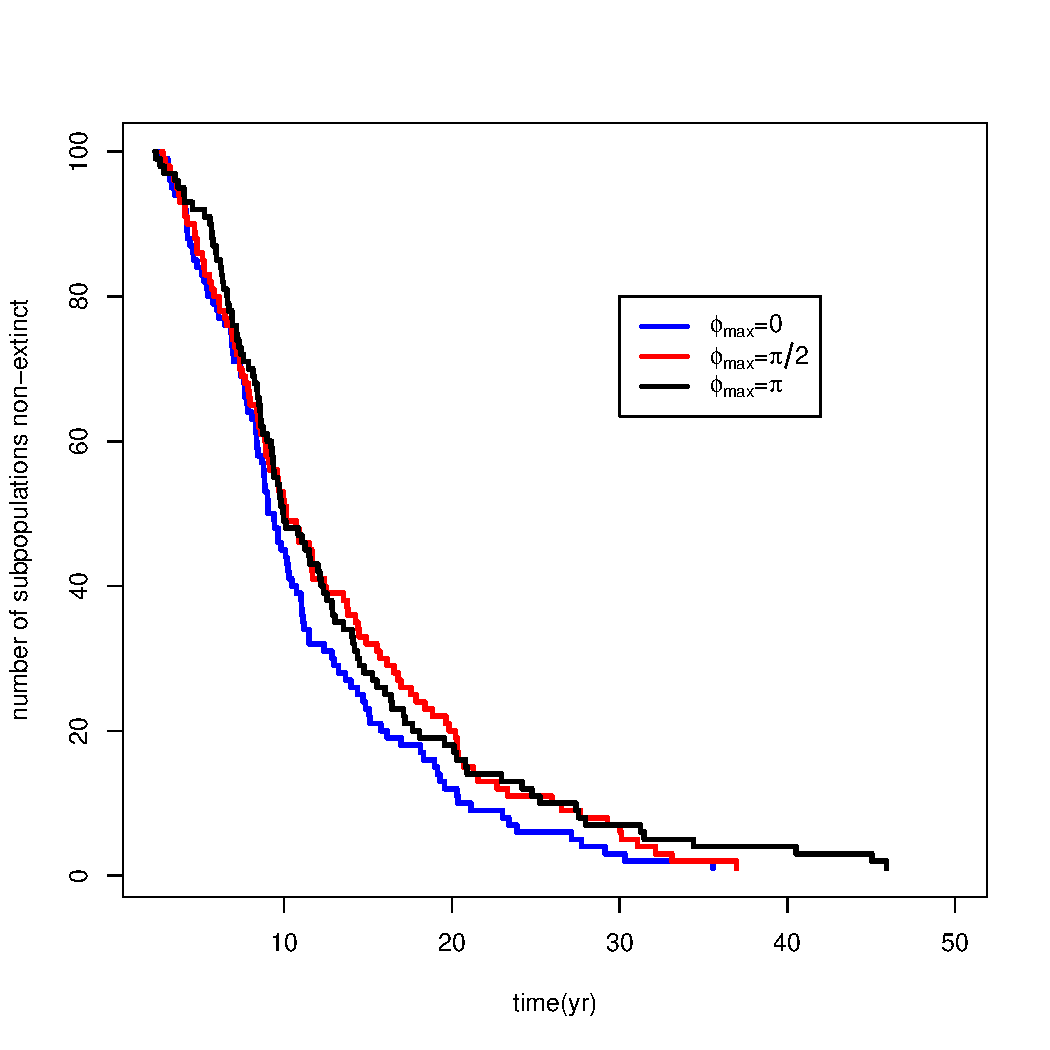
\includegraphics[scale=0.4]{smRep100Vil02R001N3e5} \caption{Kaplan-Meier survival curves for disease persistence after 100 different
simulations of $\varphi_{max}=0$, $\varphi_{max}=\pi/2$ and $\varphi_{max}=\pi$.
The blue survival curve for $\varphi_{max}=0$, the red survival curve
for $\varphi_{max}=\pi/2$ and the black curve for $\varphi_{max}=\pi$.
The disease persistence time of $\varphi_{max}=0$ is the shortest.
This of $\varphi_{max}=\pi$ is the longest.}


\label{fig:persm100phi0pi2pi_01} 
\end{figure}


The phase of forcing of the $subpopulation_{1}$ is always fixed at
$0$, but that of the $subpopulation_{2}$ increases from $0$ to
$\pi$. It means that, in the first experience, $\varphi_{max}=0$,
the two subpopulations are in synchrony with all beginning conditions.
The disease persistence time is the shortest. Then, the two subpopulations
become asynchronous when $\varphi_{max}=\pi/2$ or $\pi$. The symmetry
of fixed points is just broken at the starting moment. It is the reason
why the level of synchrony of the metapopulation decreases. Additionally,
we find that the value of the asynchrony parameter $\varphi_{max}$
change according to increasing tendency, the phase difference between
the fluctuations of the two infection rates $\beta$ augments also,
and the global persistence time in the metapopulation thus goes up.
When \textbf{$\varphi_{max}=\pi$, }the two subpopulations are in
antiphase. The balance points at the begining moment of $subpopulaiton_{1}$
are inverse to that of $subpopulation_{2}$, it accounts for why the
two subpopulations take a long duration to obtain the balance state.
This is the most difficult case to find global extinction, the persistence
time is the longest. Moreover, theses results are explicated by recolonization
between the two subpopulations. When the disease no longer exists
in one subpopulation at the moment $t$. If at this moment, the neighbouring
subpopulation obtains also the extinction, so we have a global extinction
in the metapopulation and the disease is entirely extinct. However,
in a metapopulation, due to different factors for migration between
subpopulations, we hardly see extinction at the same time in all subpopulations
in first duration. The infected in other subpopulation migrates to
the extinct subpopulation, so the disease is active. It is the reason
why the disease exists for long term. In short, the level of synchrony
between subpopulation is stronger, metapopualtion is easier to find
global extinction. Make all subpopulations synchronize is the easiest
way at which disease goes to extinct.

Additionally, we have done also experiences for local fluctuations
of subpopulations. Here, local fluctuations is called local dynamics
or local noises. It is an important factor that can increase local
extinction numbers but make global extinction rate reduce as the following
figure\textbf{ \ref{fig:nbExtAvrVil02}}.

\begin{figure}[tbph]
\centering 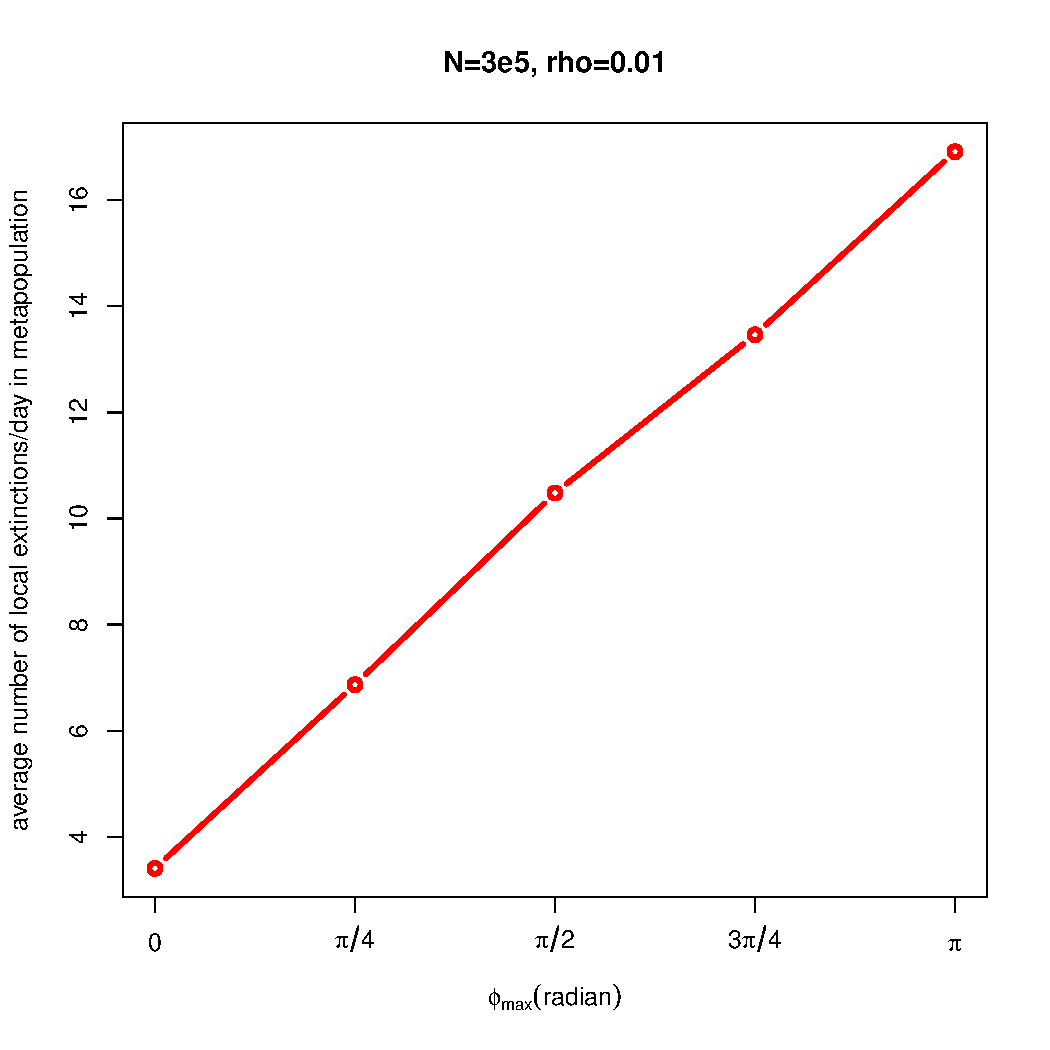
\includegraphics[scale=0.4]{nbExtAvrN3e5Rho001} \caption{Average number of local extinctions in the metapopulation of two subpopulations
and the level of synchrony after 100 different simulations. In this
figure, both the level of asynchrony increases from 0 to $\pi$ and
the number of local extinctions augments. }


\label{fig:nbExtAvrVil02} 
\end{figure}


As illustrated above, global persistence rate is inversely proportional
to global extinction rate. The global persistence rate increases,
it is synonymous with a reduction of global extinction rate. Thus,
from the figure \textbf{\ref{fig:nbExtAvrVil02}}, the number of local
extinctions in the metapopulaiton scales inversely global extinction
rates. Because of the local noises, subpopulations become extinct
but are always recolonized in short time. Local correlation between
subpopulations is soul of synchrony in metapopulation. We use local
correlation to measure level of synchrony and through that we estimate
probabilities of global extinction.


\subsection{Quantifying global persistence and asynchrony level $\varphi_{max}$}

As mentioned about, we use survival regression model for global peristence
curve to estimate its global extinction rate and to quantify persistence
level for each value $\varphi_{max}$ with confidence interval 95\%.
The result below is pointed for the metapopulation of eight subpopulations,
the population sise of each subpopulation $N=3\times10^{5}$ and the
coupling rate $\rho=0.1$ as following figure \ref{fig:perrateVil06Rho001n1e5}.

\begin{figure}[tbph]
\centering 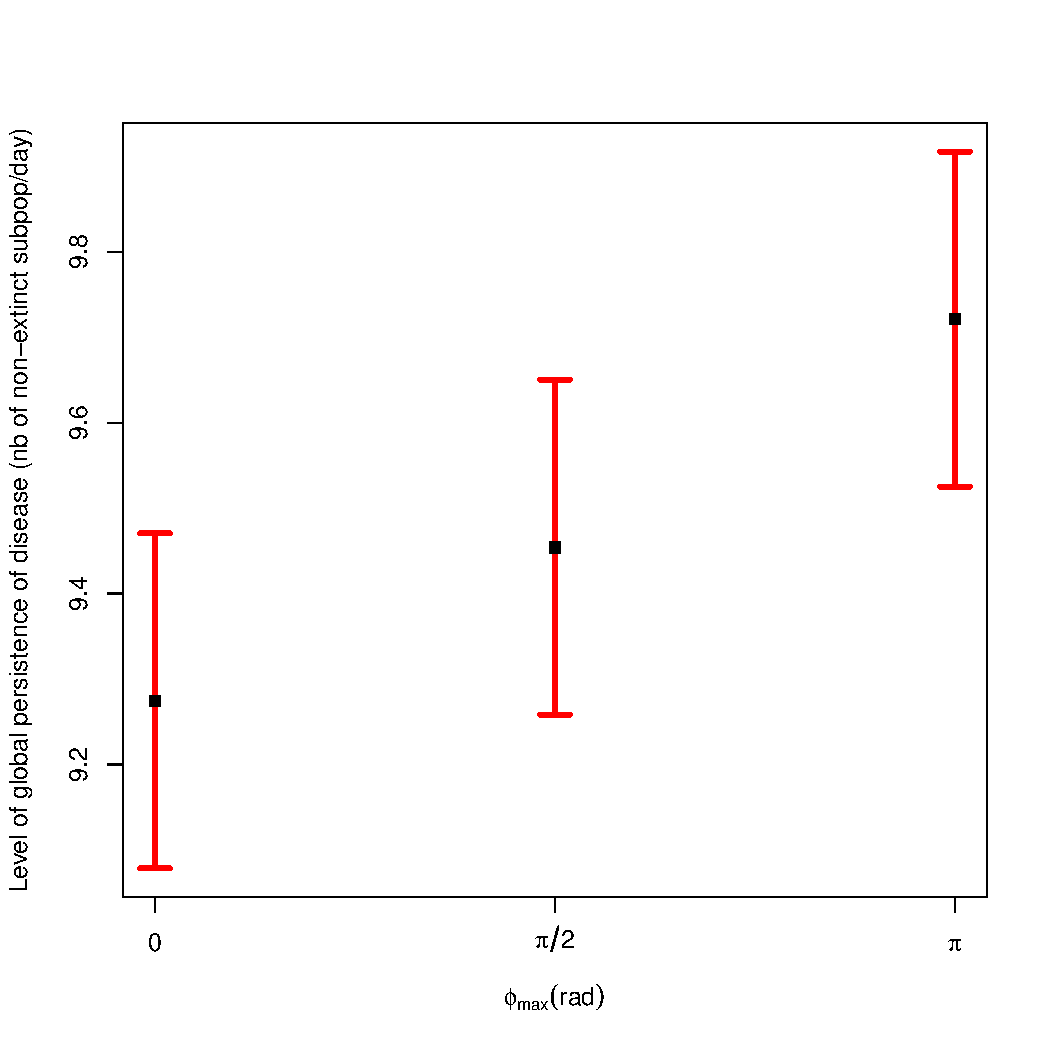
\includegraphics[scale=0.4]{resMetaPop08N3e5Rho01Rep100}
\caption{Estimated level of global disease persistence in the metapopulation
of the eight subpopulations after 100 different simulations $N=3\times10^{5}$,
coupling rate $\rho=0.1$. Here, with 95\% confidence interval, blue
lines are confidence intervals for persistence rate of each value
of $\varphi_{max}$. This intervals are limited by lower and upper
confidence limits.}


\label{fig:perrateVil06Rho001n1e5} 
\end{figure}


This figure \ref{fig:perrateVil06Rho001n1e5} shows to us that the
amplitude of the confidence intervals for each value of $\varphi_{max}$
are quite far to each other. Furthermore, it rises robustly when $\varphi_{max}$
runs from $0$ to $\pi$. The phase difference strongly influences
disease persistence time as well as global disease persistence level.
Figure \ref{fig:perrateVil06Rho001n1e5} indicates the trend of level
of persistence with increasing level of asynchrony. The asynchrony
between subpopulations is the main reason why the infectious disease
has never been extinct.

\bigskip{}


In order to press the strong dependence of the global disease persistence
to the asynchrony level parameter $\phi_{max}$, here we introduce
the results of the metapopulations of many different subpopulations.
First, we study levels of disease persistence in metapopulations of
six, ten and twenty subpopulations with population size of each subpopulation
$N=3\times10^{5}$ and the coupling rate \textbf{$\rho=0.01$}. We
obtain also the same result as the metapopulation of eight subpopulations
(figure \ref{fig:confintVil3510Rho0001N2e5}), when the level of asynchrony
$\varphi_{max}$ increases, so the persistence of disease augments.
On the other hand, the probability of disease persistence also alters
with the different numbers of subpopulation. In this result (figure
\ref{fig:confintVil3510Rho0001N2e5}), the global persistence of the
six subpopulations is minimum and that of the twenty subpopulations
is maximum.

\begin{figure}[tbph]
\centering 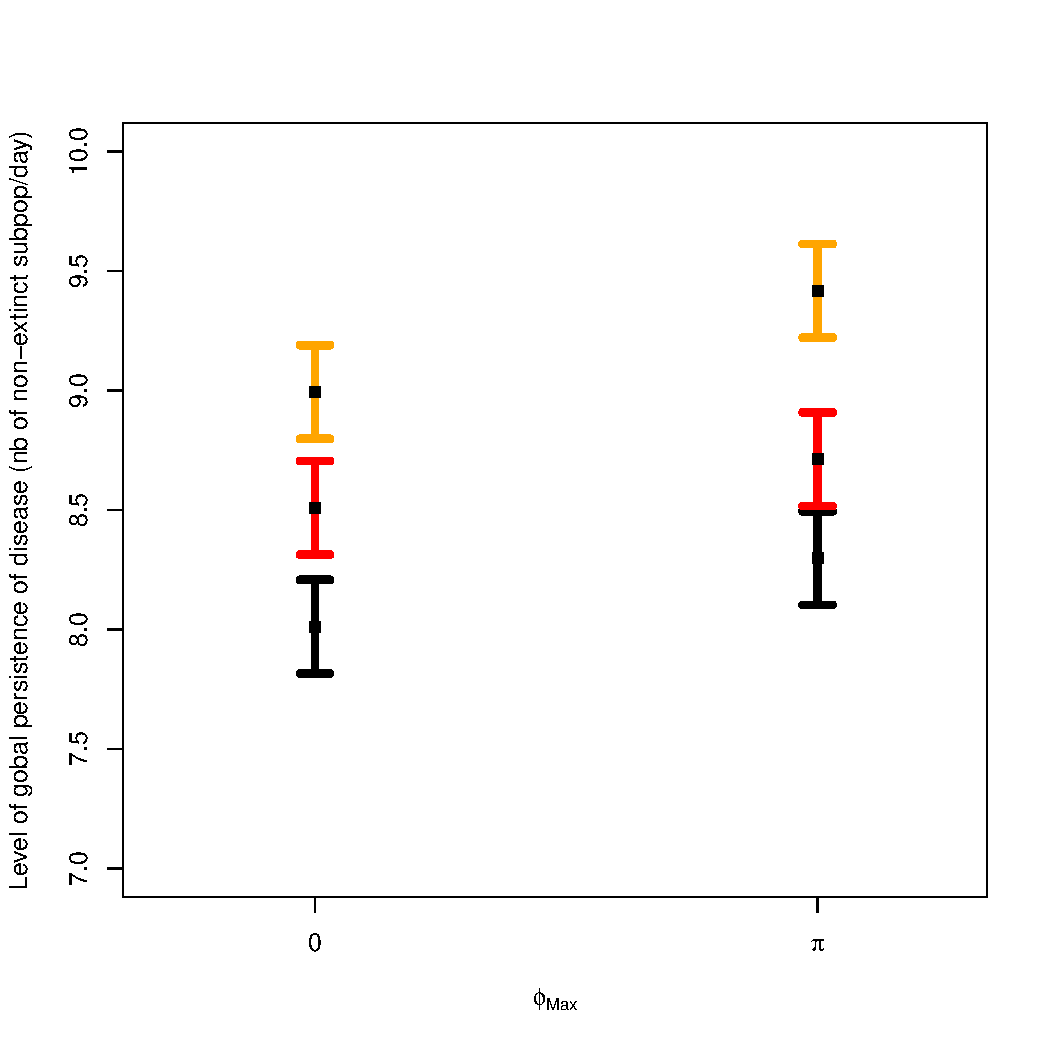
\includegraphics[scale=0.4]{resVil61020Rho001N1e5} \caption{Estimated level of persistence in the metapopulation of six, ten and
twenty subpopulations after 100 different simulations. Here, with
95\% confidence interval, black, red, and orange lines are for six,
ten and twenty subpopulations, respectively. These intervals are limited
by lower and upper confidence limits. }


\label{fig:confintVil3510Rho0001N2e5} 
\end{figure}



\subsection{Influence of other parameters on global disease persistence}


\subsubsection{Number of subpopulation in a metapopulation}

In this part, we developed the relation between the disease persistence
and the number of subpopulations in a metapopulation. We performed
simulations with metapopulations from three to 30 subpopulations,
population sizes of each subpopulation $N=10^{5}$ and $\varphi_{max}=\pi$.
The result as following figure \textbf{\ref{fig:perrateMultVil}}.

\begin{figure}[tbph]
\centering 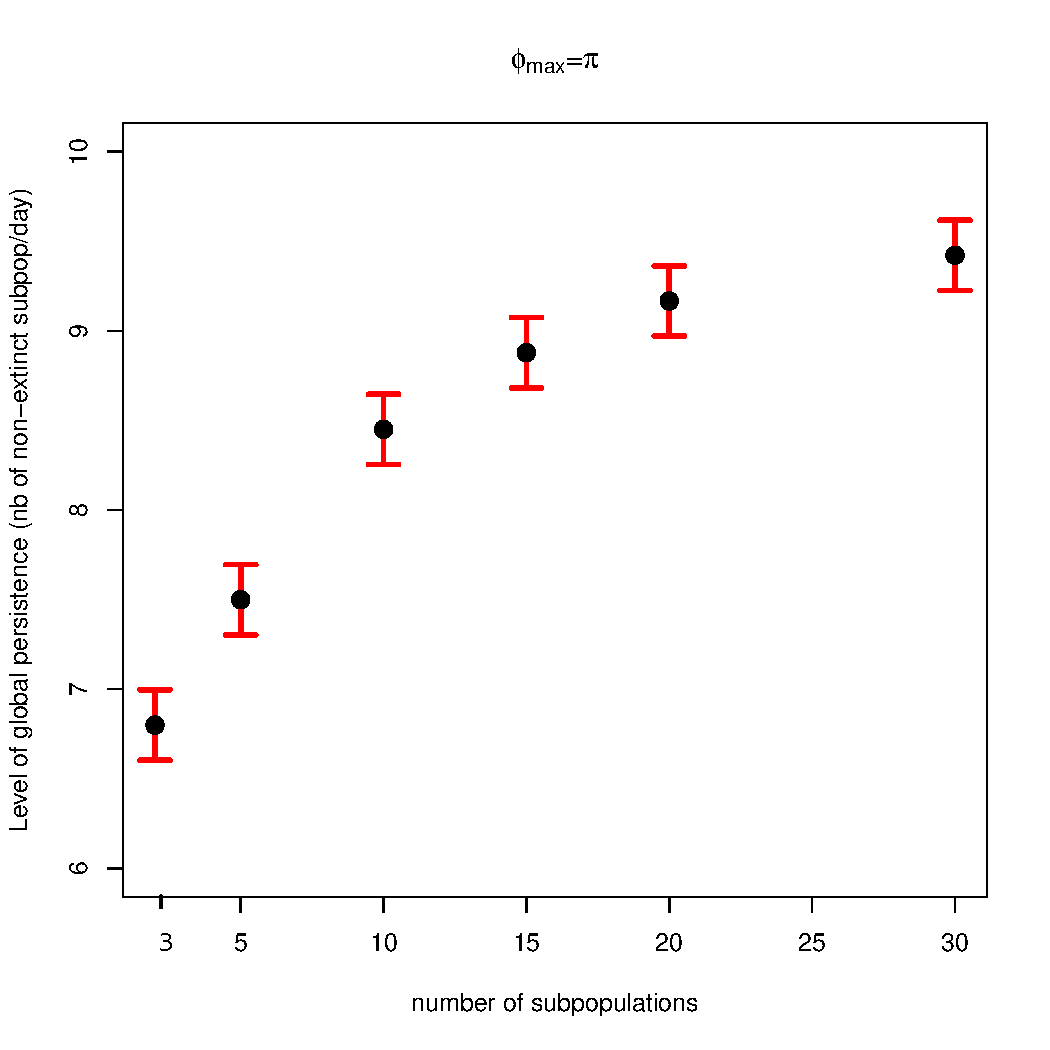
\includegraphics[scale=0.4]{resMetaPop35710152030N1e5Rho0001Rep100}
\caption{Level of disease persistence in the metapopulation of many subpopulations
with $\varphi_{max}=\pi$ and $\rho=0.001$. The number of subpopulation
is from three to 30.}


\label{fig:perrateMultVil} 
\end{figure}


The result exhibits to us that the number of subpopulations strongly
has an influence for the disease persistence time. The global persistence
level of an infectious disease in a metapopulation increases when
the number of subpopulations in this metapopulation increases. As
this is a coupling model, there are an interaction among subpopulations.
The number of subpopulation increases, influence degree of neighbouring
subpopulation on $subpopulation_{i}$ is more and more complex and
strong. The probability of disease recolonization of $subpopulation_{i}$
also rises, thereby the disease persistence increases.


\subsubsection{Population size of each subpopulation in a metapopulation}

In the metapopulation of 06 subpopulations, we implemented experiences
with different population sizes of subpopulation. We performed 100
different simulations for the metapopulation of 06 subpopulations
in which all subpopulations has the same population size N. We set
N from $5\times10^{3}$ to $5\times10^{5}$ individuals. The result
(figure \textbf{\ref{fig:perrateMultVil-1-1}}) affirms that the population
size influences strongly the global persistence of an infectious disease
in a metapopulation. The number of individuals in a subpopulation
grows, so the global persistence of disease increases also.

\begin{figure}[tbph]
\centering 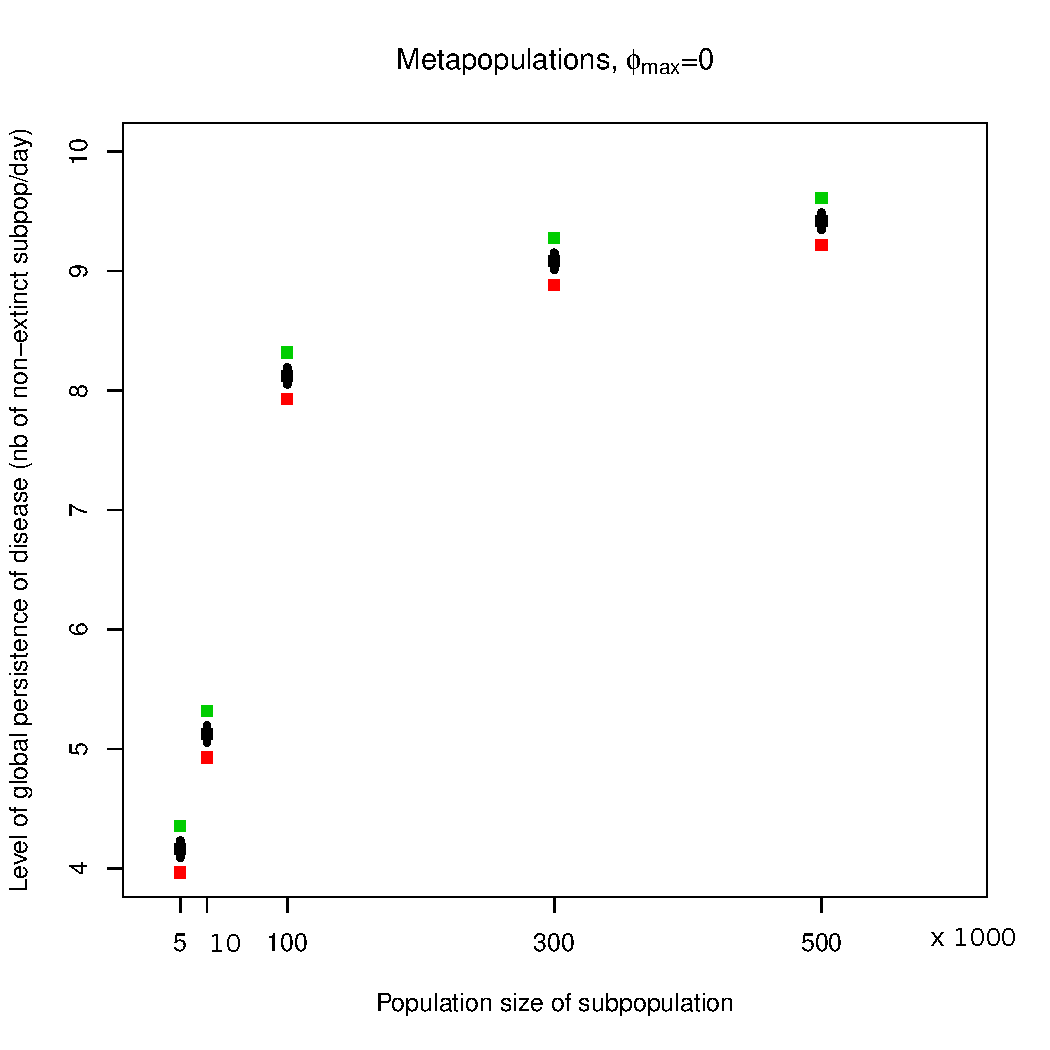
\includegraphics[scale=0.4]{resMeta06rho01NChangephi0}
\caption{Relation between level of global disease persistence and the population
size of each subpopulation. With 95\% confidence interval, the red
points are lower limites and the green points are upper limites. Here,
the number of subpopulation is six, the coupling rate $\rho$ is $0.1$,
the level of asynchrony $\varphi_{max}$ is \{0\} and the population
size of each subpopulaiton N is in \{$5\times10^{3}$,$10\times10^{3}$,$100\times10^{3}$,
$300\times10^{3}$,$500\times10^{3}$\}.}


\label{fig:perrateMultVil-1-1} 
\end{figure}


From the result (figure \ref{fig:perrateMultVil-1-1}), the population
size and the global persistence of disease are directly proportional.
This is effect of the inscrease of population size that is reason
for that the number of infectives present augments, and therefore
both the demographic stochasticities and probability of global extinction
decrease.


\subsubsection{Coupling rate}

One more factor that was pointed in the introduction part is coupling
strength between subpopulations. Here, the coupling rate or the dispersal
rate $\rho$ can be considered as migration strength. The disease
transmission speed grows fast when coupling rate goes up in metapopulations.
Similar to that, global disease persistence surges also. In this part,
we permit coupling rate change from weak to strong in a metapopualtion
of five subpopulations with the population size $N=10^{5}$ for each
subpopulation. The dispersal rate $\rho$ is divided into three intervals.
These are low, intermediate and high coupling rate intervals. In each
interval, we chose some coupling rates that highlight the coupling
strength among subpopulations in a metapopulation.\textbf{ }With each
value of coupling rate, we estimated gradient coefficient for the
relation between persistence level of disease and level of asynchrony
$\varphi_{max}$, in condition $\varphi_{max}$ belonging to the set
\{0, $\pi/2$, $\pi$\}. Now, we have result as following figure \ref{fig:perrateMultVil-1-1}.

\begin{figure}[tbph]
\centering 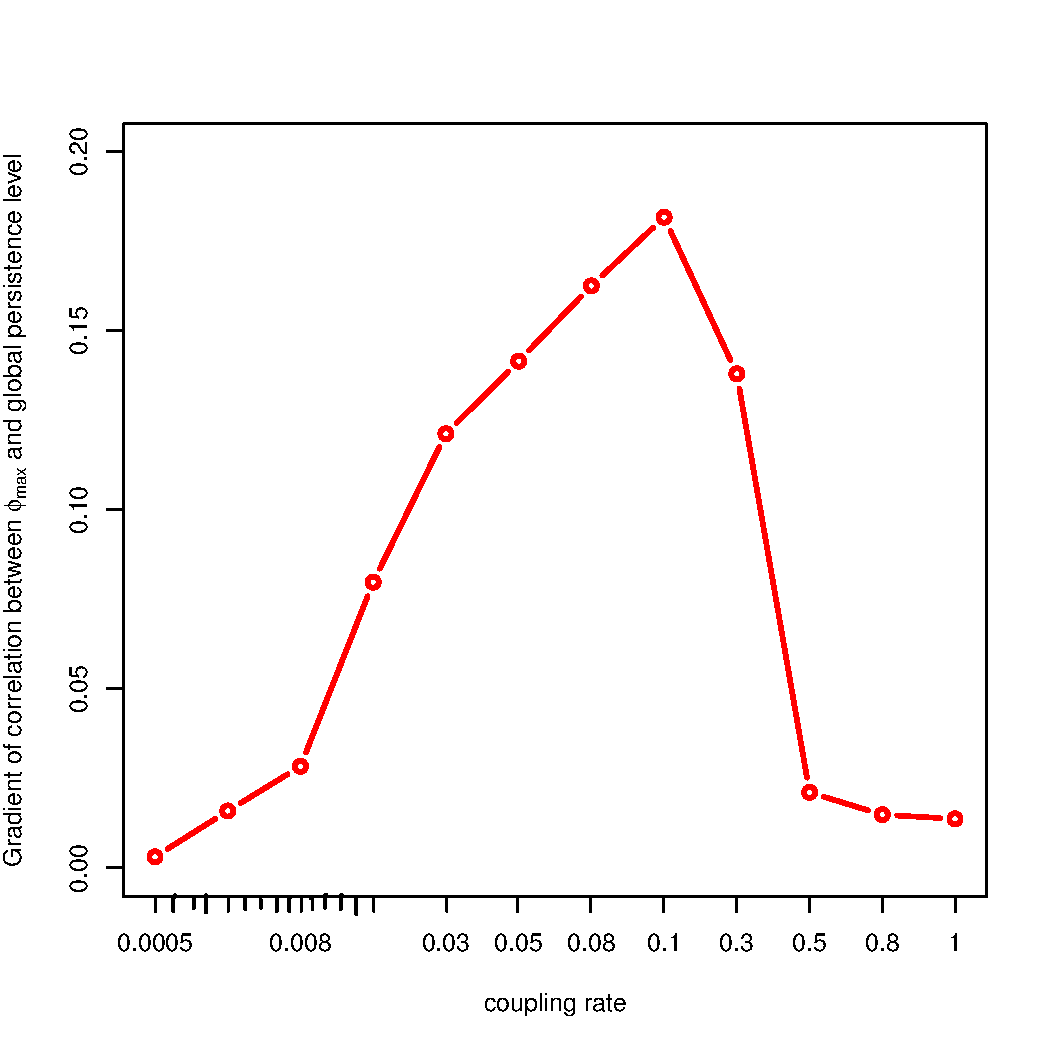
\includegraphics[scale=0.4]{resPenteVil05multiRho_2}
\caption{Correlation between coupling rate and gradient of level of synchrony
and persistence rate in the metapopulation of five subpopulation.
Here, the coupling rate $\rho$ is in \{0.0005,0.001,0.008,0.01,0.03,0.05,0.08,0.1,0.3,0.5,0.8,1\},
the level of synchrony $\varphi_{max}$ in \{0,$\pi/2$ ,$\pi$\}
and the population size of each subpopulaiton N=1e5.}


\label{fig:resPenteVil05multiRho-1} 
\end{figure}


When the coupling rate is small from 0.0005 to 0.008, the gradient
of the correlation between $\varphi_{max}$ and the global persistence
increases very slowly. However, the persistence level augments in
a sudden way when the coupling rate changes from 0.01 to 0.1. Lastly,
the gradient strongly decreases when the coupling rate is so robust
from 0.3 to 1.0. Based on this figure, the global disease persistence
in a metapopulation is one humped function for the coupling rate.
The medium coupling rate (from 0.01 to 0.1) maximizes disease persistence
in metapopulation. As in the case of the small and average coupling
rates, the coupling rate and the speed of migration among subpopulations
are directly proportional. The dispersal speed increases, thereby
the local recolonization speed rises, the duration of persistence
grows. However, this trend of global persistence with increasing coupling
rate, is not right any more when the dispersal rate is strong. The
duration of persistence falls, because the metapopulation has tendency
to become one big population. In this case, the phase difference or
the recolonization among subpopulations are no longer significant.


\section{Discussion and Conclusion}

We successfully have built a version for the susceptible-infectied-recovered
stochastic metapopulation model. The infection rate $\lambda_{i}$
for \textbf{$subpopulation_{i}$ }has portrayed all effects inside
as well as outside of the disease tranmission chain between individuals
in the same subpopulation or in other subpopulations. Moreover\textbf{,
}our metapopulation model became more detailed when we brought seasonality\textbf{
}in metapopulation model to create periodic transmission in year that
highlighted seasonal changes as well as school period of children
\cite{Bolker1993,Bolker1995,Earn1998,Keeling2002}\textbf{. }We have
metapopulation model with different contact rates for each subpopulation.
This is a more complex model than any used metapopulation model. We
have sketched successfully in-phase and sometime out-of-phase (``antiphase'')
models across suburbs of He's 2003 \cite{He2003}

This complex metapopulation model is also an expected result of Rozhnova(2012)
\cite{Rozhnova2012}. It's a good result for scientists wanting to
use the SEIR metapopulation model for simulating dynamics of infectious
diseases. Our results roughly support those of Rozhnova's 2012. The
authors gave different values of the contact rates $\beta$ of each
subpopulation. However, the rates $\beta$ here are fixed by constants
and the number of subpopulations in experiences are maximum of three.
Comparing this result with our's, in a coupling metapopulation, the
degree of synchorny is maintained when the coupling rate between subpopulations
is weak.

Moreover, our stochastic SEIR metapopulation model with subpopulations
connected to each other, we have quantified disease persistence of
seasonality as well as spatial synchrony. With our model, we can easily
create level of seasonality in year and at the same time, phase difference
in seasonality between subpopulations. It's the reason why we have
model quite close to the metapopulation model in reality.

Due to the phase difference between infection coefficient $\beta$,
we can change by an increase or a decrease in level of synchrony.
We want to decrease level of synchrony, by simply increasing the phase
difference between forcing phase coefficients in the formulas of contact
rate $\beta$. Clearly, the level of synchrony between two subpopulations
are the worst when the two fluctuations are in antiphase (as figure
\ref{fig:persm100phi0pi2pi_01}). When the phase difference between
oscillations increases, the desynchronizing effect on population dynamics
of the subpopulations augments. This enhances disease persistence
time though the global extinction rate is reduced. Moreover, as the
result above (figure \textbf{\ref{fig:nbExtAvrVil02}}), in the local
shape,\textbf{ }our result, along with those of Bolker (1995) \cite{Bolker1995}
and Heino (1997) \cite{Heino1997}, stress the number of local extinctions\textbf{
}being inversely proportionnel with the global extinction rate in
a metapopulation. When the level of synchrony is at a reduction and
the global persistence time gets an increase, the global extinction
rate of metapopulation goes down and the number of local extinction
goes up. Due to the result about local extinction, we also affirm
that disease is always available in metapopulation if and only if
at least one subpopulaiton is not extinct.\textbf{ }

Our finding has specified the two main factors influencing the persistence
ability of an infectious disease. One factor is transmission characteristics
of the infectious disease and the other is interplay between mixing
subpopulations in metapopulation. The interaction between the disease
persistence and the spatial heterogeneity becomes a major key to unlock
questions about infectious disease in epidemiology. This result takes
a large part in epidemic disease persistence domain that has being
exploited in scientific epidemically research works. We gained a robust
understanding of how disease persistence is affected by local factors
such as spatial heterogeneity, demographic asynchrony and seasonality,
as well as mixing factors such as migration, disease transmission
between hosts and pathogens. Lastly, we also highlighted recolonization
effects. It is like rescue for disease. Because of connection between
subpopulation, individuals can go everywhere. Subpopulation is quickly
re-infected althought the disease has became extinct. Thus, the disease
rescus makes local extintions difficult to extend into global extinctions.

As a matter of the fact of coupling strength among subpopulations
in metapopulation, we proved that\textbf{ }the persistence of the
disease in the metapopulation is not only a exponential survival function
over time, but also a humped function for the coupling rate. In addition,
the global disease persistence in metapopulation is maximum when the
coupling rate between subpopulations is just medium. This finding
is similar to those of Huffaker(1958) \cite{huffaker1958experimental},
Holyoak and Lawler(1996) \cite{holyoak1996persistence}, and Yaari
et al. (2012) \cite{Yaari2012} when they exhaustively explored the
disease persistence behavior of many different metapopulation models.
And our result one more time affirms that the disease persistence
and the interaction in metapopulation models are significant when\textbf{
}the interaction strength $\rho$ is from $10^{-3}$ to 0.1 \cite{KeelingRohani2008}.

To summarize, we have built successfully a\textbf{ }sinusoidally forced
SEIR stochastic metapopulation model. This model is like a physical
system of coupled oscillators. We have pointed out that spatial synchronization
consistently and predictably makes extinction risk increase by using
the model 0 where all the subpopulations have the same population
size $N$ and there is no explicit spatial distance. So, it's good
for the future, we can continue this work with different population
size of each subpopulation and different spatial distance between
subpopulations and then, create synchronous metapopulations that optimize
vaccination policies.

\bibliographystyle{plain}
\bibliography{bikBokEpidemics,bikCCS,bikPerSyns}


\newpage{}


\section*{Appendix : equilibrium values of the system \ref{eq:dS}--\ref{eq:dR}}

We start with ordinary differential equations for a $subpopulation_{i}$
in a metapopulation as follows:

\begin{eqnarray}
\frac{dS_{i}}{dt} & = & \mu N_{i}-\lambda_{i}S_{i}-\mu S_{i}\\
\frac{dE_{i}}{dt} & = & \lambda_{i}S_{i}-\mu E_{i}-\sigma E_{i}\\
\frac{dI_{i}}{dt} & = & \sigma E_{i}-\mu I_{i}-\gamma I_{i}\\
\frac{dR_{i}}{dt} & = & \gamma I_{i}-\mu R_{i}
\end{eqnarray}
 In simulation, we know that the equilibrium state allow a disease
to persist in a population for a long time. So, an infectious disease
in the $subpopulation_{i}$ is available in long term this system
is at equilibrium. It means that at which $\frac{dS_{i}}{dt}=\frac{dE_{i}}{dt}=\frac{dI{}_{i}}{dt}=\frac{dR{}_{i}}{dt}=0$
({*}). Thus, we let all equations (equations $15$ - $18$ ) in the
system be equal to zero, then calculate the values of the variables
(now denoted by $S_{i}^{*}$, $E_{i}^{*}$, $I_{i}^{*}$ , and $R{}_{i}^{*}$)
that satisfy this condition ({*}). We have these values as folllows:

\begin{eqnarray}
S_{i}^{*} & = & N_{i}\frac{(\gamma+\mu)(\sigma+\mu)}{\beta\sigma}\\
E_{i}^{*} & = & N_{i}\mu\left(\frac{1}{\sigma+\mu}-\frac{\gamma+\mu}{\beta\sigma}\right)\\
I_{i}^{*} & = & N_{i}\mu\frac{\beta\sigma-(\sigma+\mu)(\gamma+\mu)}{\beta(\sigma+\mu)(\gamma+\mu)}\\
R_{i}^{*} & = & N_{i}-S_{i}^{*}-E_{i}^{*}-I_{i}^{*}
\end{eqnarray}


Here, if we set $R_{0}=\frac{\beta\sigma}{(\gamma+\mu)(\sigma+\mu)}$,
so we have

\begin{eqnarray}
S_{i}^{*} & = & N_{i}\frac{1}{R_{0}}\\
E_{i}^{*} & = & N_{i}\frac{\mu\sigma}{R_{0}}\left(R_{0}-1\right)\\
I_{i}^{*} & = & N_{i}\frac{\mu}{\beta}(R_{0}-1)\\
R_{i}^{*} & = & N_{i}-S_{i}^{*}-E_{i}^{*}-I_{i}^{*}
\end{eqnarray}


One nomal conditions for all population availabes is that the equilibrium
values cannot be negative. Therefore, an infectious disease is available
in the $subpopulation_{i}$ if $R_{0}>1$. Now, the endemic equilibrium
in the system is given by $(S_{i}^{*},E_{i}^{*},I{}_{i}^{*},R{}_{i}^{*})$
= $(N_{i}\frac{1}{R_{0}}$, $N_{i}\frac{\mu\sigma}{R_{0}}\left(R_{0}-1\right)$,
$N_{i}\frac{\mu}{\beta}(R_{0}-1)$, $N_{i}(1-\frac{1}{R_{0}}-\frac{\mu\sigma}{R_{0}}\left(R_{0}-1\right)-\frac{\mu}{\beta}(R_{0}-1))$.\newpage{}


\section*{Appendix: derivation of the equation \ref{eq:force-1}}

We assume that the infection process is frequency-dependent, meaning
that the force of infection $\lambda$ is proportional to a proportion
of infected: $I/N$. Infection of susceptibles from one population
$i$ can be due to contacts with infected from the same population
$i$ or to contacts with infected from another population $j$. In
the first case, the force of infection simply reads 
\begin{equation}
\lambda_{i,w}=\beta_{i}\frac{I_{i}}{N_{i}}\label{eq:w}
\end{equation}
 where $\beta$ is the infectious contact rate in population $i$. 

In the second case, susceptible individuals from population $i$ can
be infected through contacts with infected individuals from population
$j$ in two different manners: either the susceptible individuals
from population $i$ visit population $j$ and get infected there
before coming back to their population of origin $i$, or infected
individuals from population $j$ that visit population $i$ and infect
susceptible individuals from this population $i$ before going back
to their population of origin $j$. In the first case, the total rate
of transmission to the entire susceptible group of population $i$
visiting population $j$: 
\begin{equation}
\lambda_{i,b_{s}}=\beta_{j}\frac{I_{j}}{N_{j}}\label{eq:bs}
\end{equation}
 and in the second case the force of infection reads 
\begin{equation}
\lambda_{i,b_{i}}=\beta_{i}\frac{I_{j}}{N_{i}}.\label{eq:bi}
\end{equation}


Note that in this study we are interested in the spatial dynamics
of the disease, not of the host individuals on which the spread of
disease (we assume for that that the visits of individuals to other
populations are always of short duration). Movements of individuals
are thus not explicitly modeled, only the spatial dynamics of the
infection process is modeled. Combining equations \ref{eq:bs} and
\ref{eq:bi}, the force of infection due to contacts with infected
individuals from another population $j$ reads 
\begin{eqnarray}
\lambda_{i,b} & = & (1-\varepsilon_{ij})\lambda_{i,b_{s}}+\varepsilon_{ij}\lambda_{i,b_{i}}\\
 & = & (1-\varepsilon_{ij})\beta_{i}\frac{I_{j}}{N_{i}}+\varepsilon_{ij}\beta_{j}\frac{I_{j}}{N_{j}}\\
 & = & \frac{(1-\varepsilon_{ij})\beta_{i}N_{j}+\varepsilon_{ij}\beta_{j}N_{i}}{N_{i}N_{j}}I_{j}\label{eq:b}
\end{eqnarray}
 where $\varepsilon_{ij}=\varepsilon_{ji}$ ($0\leqslant\varepsilon_{ij}\leqslant1$)
is the proportion of susceptible individuals from population $i$
visiting population $j$ being infected with population $j$ and $1-\varepsilon_{ij}=1-\varepsilon_{ji}$
is the proportion of susceptible individuals from population $i$
being infected due to infected individuals from population $j$ visiting
population $i$. Now, combining equations \ref{eq:w} and \ref{eq:b},
we can express the force of infection in population $i$, accounting
for another population $j$: 
\begin{equation}
\lambda_{i}=(1-\rho_{ij})\beta_{i}\frac{I_{i}}{N_{i}}+\rho_{ij}\frac{(1-\varepsilon_{ij})\beta_{i}N_{j}+\varepsilon_{ij}\beta_{j}N_{i}}{N_{i}N_{j}}I_{j}
\end{equation}
 where the coupling coefficient $\rho_{ij}=\rho_{ji}$ ($0\leqslant\rho_{ij}\leqslant1$)
is the proportion of interactions that occurs between populations
$i$ and $j$. We can generalize the above equation to the case of
$n$ populations: 
\begin{equation}
\lambda_{i}=\left(1-\sum_{\substack{k=1\\
k\neq i
}
}^{n}\rho_{ik}\right)\beta_{i}\frac{I_{i}}{N_{i}}+\sum_{\substack{k=1\\
k\neq i
}
}^{n}\rho_{ik}\frac{(1-\varepsilon_{ik})\beta_{i}N_{k}+\varepsilon_{ik}\beta_{k}N_{i}}{N_{i}N_{k}}I_{k}
\end{equation}


By resuming the formula $\lambda_{i}$, we have:

\begin{equation}
\lambda_{i}=\beta_{i}\frac{I_{i}}{N_{i}}+\sum_{\substack{k=1\\
k\neq i
}
}^{n}\rho_{ik}\left[\frac{\beta_{i}\text{[}(1-\varepsilon_{ik})I_{k}-I_{i}]}{N_{i}}+\frac{\varepsilon_{ik}\beta_{k}I_{k}}{N_{k}}\right]\label{eq:force-1-1}
\end{equation}


We can verify that the cases one single population $i$ and $n$ independent
populations (i.e. with $\rho_{ik}=0$, $\forall i$ and $k$ $\neq i$)
respectively yield 
\begin{equation}
\lambda_{i}=\beta_{i}\frac{I_{i}}{N_{i}}
\end{equation}
 and 
\begin{equation}
\lambda_{k}=\beta_{k}\frac{I_{k}}{N_{k}}.
\end{equation}


\newpage{}


\section*{Appendix: supplementary materials}

Here, we present some results of the simulation with the conditions
as the same for all initial values of variables, for all parameters
of the metapopulation of two subpopulations without the synchrony
parameter $\varphi_{max}$. We let $\varphi_{max}$belong to the set
\{0, $\pi/2$, $\pi$\}. The results are shown in Figure \ref{fig:smphi00-1},
\ref{fig:smphi0pi2-1} and \ref{fig:smphi0pi-1}.

\begin{figure}[tbph]
\centering 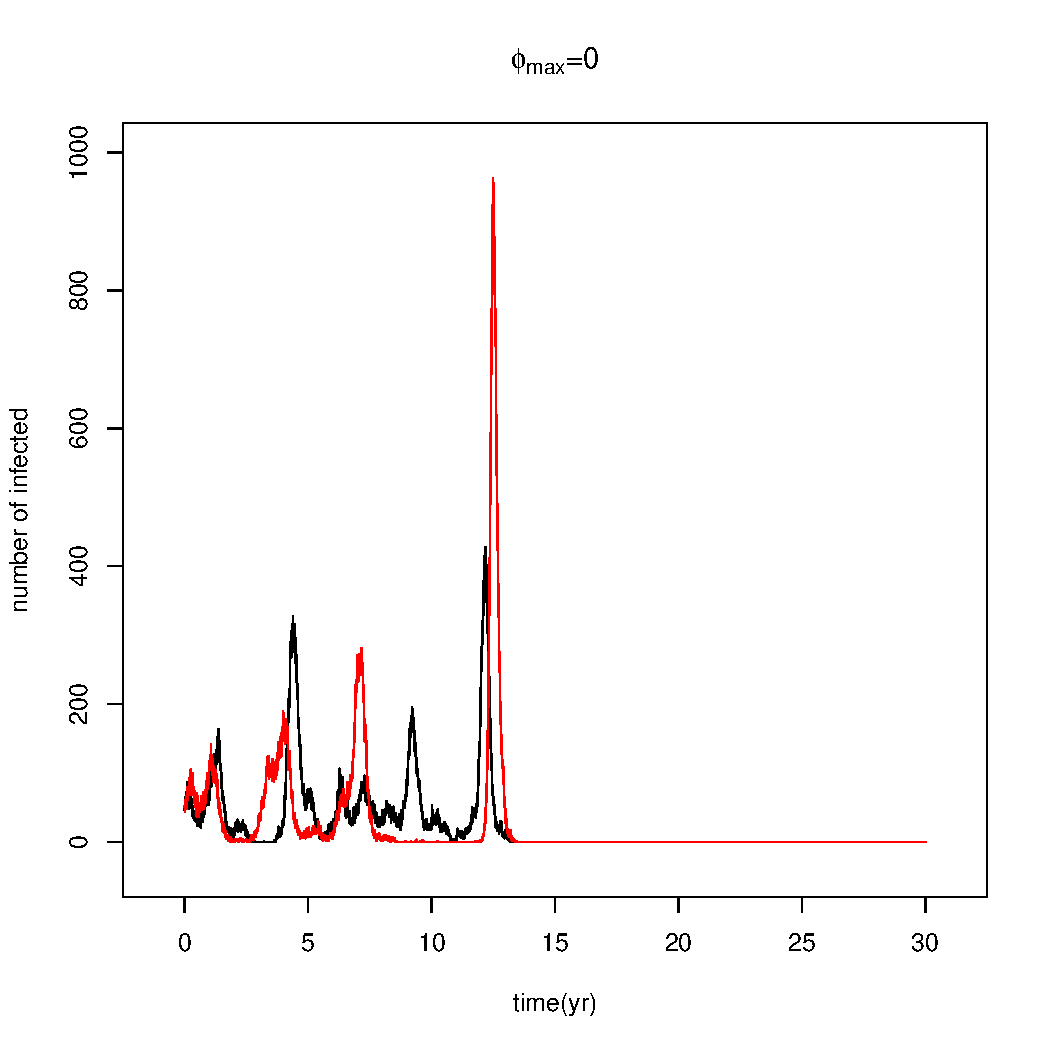
\includegraphics[scale=0.5]{smphi00Vil02Rho0001N3e5}
\caption{Metapopulation of two subpopulations in phase.\protect \protect
\protect \protect \\
 Two stochastic SEIR metapopulation model with $N_{1}=N_{2}=3\times10^{5}$,
$\rho=0.001$, $\varphi_{max}=0$ and simulation time = 30 years.
The black line for $subpopulation_{1}$ and the red line for $subpopulation_{2}$.
Because we start doing simulation with the same all beginning conditions,
so in the first period, the two subpopulations similarly fluctuate.
Because of high level of synchrony, global extinction occurs before
10th year. }


\label{fig:smphi00-1} 
\end{figure}


With $\varphi_{max}=0$, the two subpopulation are synchronous about
all starting conditions (values of all parameters, of all variables),
so we gain the synchrony at the starting steps of simulation (fig
\ref{fig:smphi00-1}). However, here is stochastic model, so the similar
fluctuations are broken, the decorrelation between two dynamics rises.
This bring a closeness to disease dynamics in reality. The metapopulation
dynamics runs from global synchronization to desynchronization and
the global synchronization in subpopulation decays over time because
of coupling strength of community structure \cite{Yan2007}. About
fifth year, the $subpopulation_{1}$gains local extinction. But, disease
comes back after a short period of time by transfer of infected individuals
from the $subpopulation_{2}$. However, due to the high degree of
synchrony between the two subpopulations, the metapopulation obtains
a global extinction. Disease can not return into this metapopulation.

\begin{figure}[tbph]
\centering 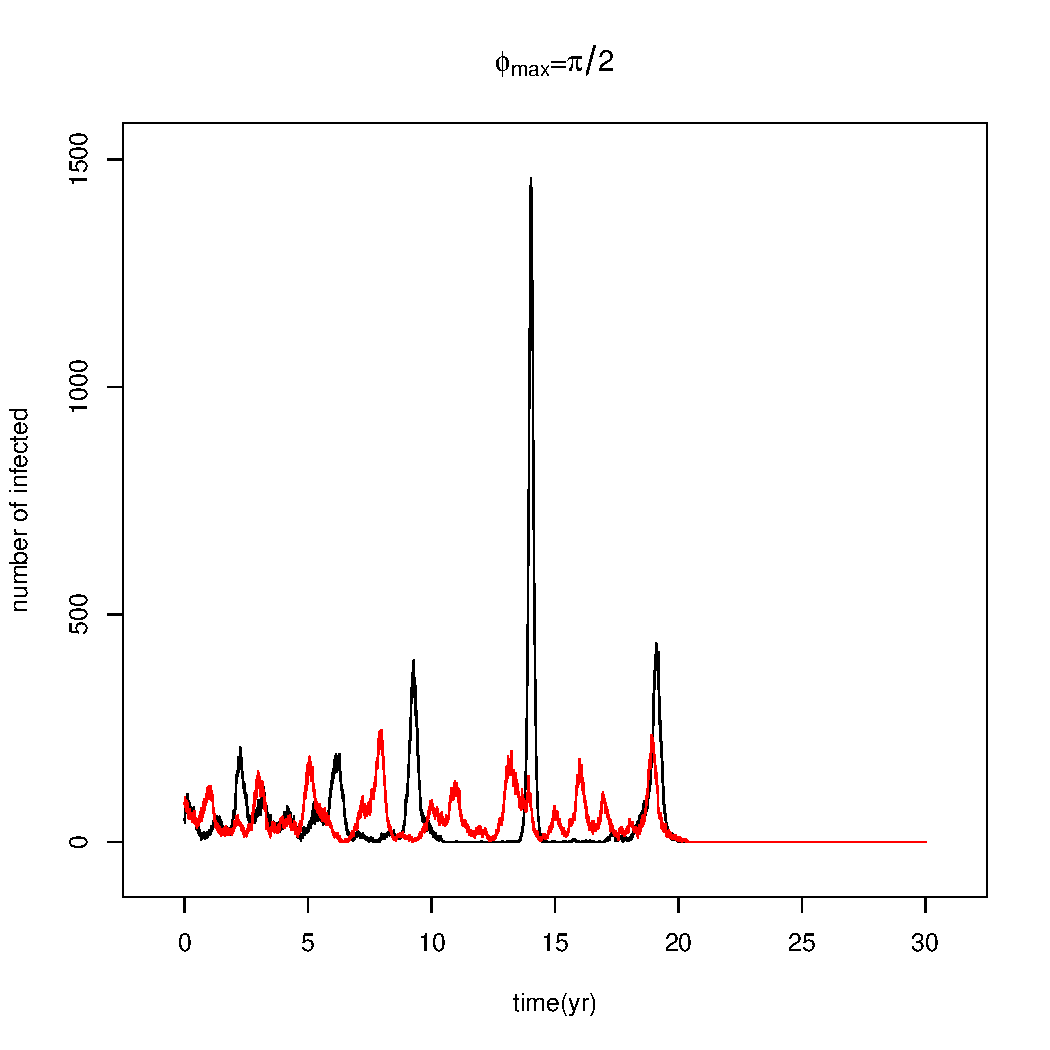
\includegraphics[scale=0.4]{smphi0pi2Vil02Rho0001N3e5}
\caption{Metapopulation of two subpopulations in phase quadrature.\protect
\protect \protect \protect \\
 Two stochastic SEIR metapopulation model with the same value for
all parameters and all variables, except $\varphi_{max}=\pi/2$. The
black line for $subpopulation_{1}$ and the red line for $subpopulation_{2}$.
The start points of the two wavelettes are out of phase and all peaks
are also always out of phase with each other. The degree of synchrony
is worse than with $\varphi{}_{max}=0$. So, the time of disease persistence
is longer. }


\label{fig:smphi0pi2-1} 
\end{figure}


Next, with $\varphi_{max}=\pi/2$, the two subpopulation are out of
phase (figure \ref{fig:smphi0pi2-1}). We give the same values for
all parameters, for all variables, but the different forcing phases,
so we gain the different contact rates. The phase difference occurs,
the synchrony structure is broken from the start moment and the number
of infected is governed by each other. In this case, the $subpopulation_{1}$gains
two times local extinction. But,\textbf{ }this subpopulation is reinfected
because disease is still availlable in the $subpopulation_{2}$. The
metapopulation gets global extinction after $15^{th}$ year. The time
of disease persistence is longer than the case \textbf{$\varphi_{max}=0$}
since the high degree of synchrony between the two subpopulations
with $\varphi_{max}=\pi/2$ is smaller than with $\varphi_{max}=0$.\textbf{ }

\begin{figure}[tbph]
\centering 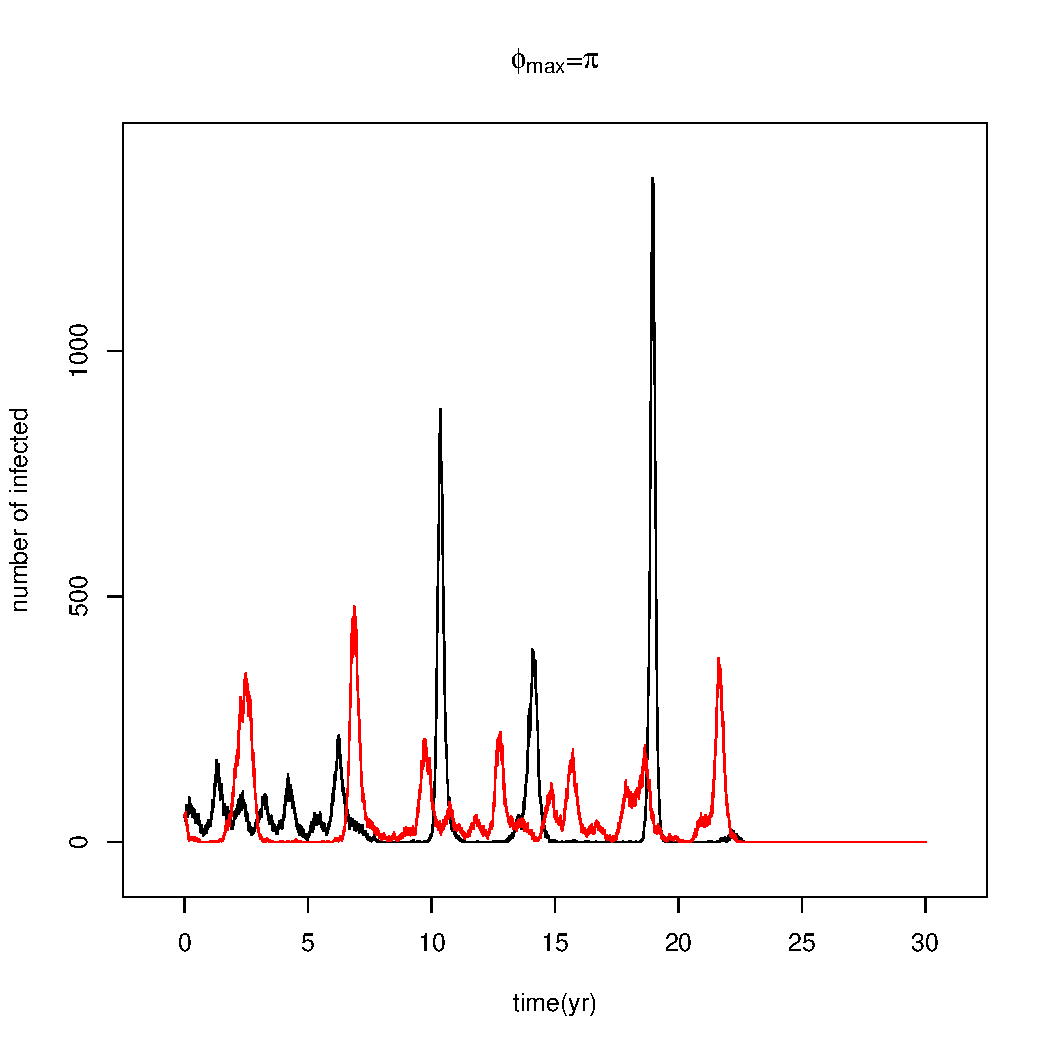
\includegraphics[scale=0.5]{smphi0piVil02Rho0001N3e5}
\caption{Metapopulation of two subpopulations in antiphase.\protect \protect
\protect \protect \\
 Two stochastic SEIR metapopulation model with the same value for
all parameters and all variables, except $\varphi_{max}=\pi$. The
black line for $subpopulation_{1}$ and the red line for $subpopulation_{2}$.
The start points of the two wavelets are in antiphase and all peaks
are also always out of phase with each other. This is the worst case,
the metapopulation finds global extinction late. }


\label{fig:smphi0pi-1} 
\end{figure}


Lastly, in the figure \ref{fig:smphi0pi-1}, we have to say that this
is the worst, global extinction have occurred latest although the
first subpopulation has gotten many times local extinction. Here,
the level of synchrony is the lowest, the phase difference is 180
degrees ($\pi$ radian). The time of persistence is the largest. However,
the phase difference with 180 degrees is step by step damped. There
are some intervals where the distance between the number of the infected
of the two subpopulations is very close to each other. So, we can
see the small phase differences between peaks of the fluctuations.
The more the phase difference increases, the more the disease persistence
time increases.

In conclusion, local extinctions are desynchronizing. This reduces
synchrony among subpopulations and promotes recolonization, and thus
causes disease persistence in long term. In the other hand, view the
figures, we can find multiyear oscilations in measles metapopulation. 
\end{document}
